\documentclass[letterpaper,twocolumn,10pt]{article}
\usepackage{iftex}
% breakurl emits PostScript hooks that XeTeX does not support. Native hyperref
% handles URLs on this engine; leave the vendored USENIX style unmodified.
\ifXeTeX
  \makeatletter
  \@namedef{ver@breakurl.sty}{2026/10/30 Native XeTeX URL handling}
  \makeatother
\fi
\usepackage{hyperref}
\usepackage{usenix}
\usepackage{xurl}
\ifXeTeX
  % XeTeX lacks these pdfTeX microtype features; retain normal font spacing.
  \microtypesetup{spacing=false,kerning=false}
\fi
\usepackage{amsmath,amssymb,booktabs,tabularx}
\usepackage{tikz}
\usetikzlibrary{arrows.meta,positioning,fit,calc}
\newcommand{\sys}{OpenAVT}
\newcommand{\code}[1]{\texttt{#1}}
\newcommand{\todoexperiment}[1]{\textit{Planned: #1}}
% Generated by paper/scripts/extract_results.py from docs/quic-verification.json.
\newcommand{\implementationcommit}{\code{033f8bf}}
\newcommand{\testcount}{226}
\newcommand{\measurementrows}{%
WebRTC PCM & None & 0.682 & 1 \\
WebRTC PCM & Fixed & 3.681 & 1 \\
Provider PCM & Fixed & 3.602 & 1 \\
WebRTC FSK & None & 35.681 & 1 \\
}

\title{OpenAVT: Binding Delegated Agent Authority to Voice Channels}
\author{Anonymous Authors\\Research draft, October 30, 2026}
\date{}
\begin{document}
\maketitle
\begin{abstract}
Personal agents increasingly act through phone calls and other perceptual interfaces.
A secure connection to an agent service does not, by itself, authorize a speaker
heard on a different channel. Voice recognition can identify a familiar synthetic
voice without establishing which customer delegated which action to its caller.
We study how to carry authenticated, scoped machine requests through the same
audio interface used for an interaction. \sys{} combines an audio modem, mutually
authenticated TLS 1.3, and a gateway that checks customer grants outside the language
model. Its QUIC variant replaces link-level reliable delivery with native QUIC
recovery over unreliable audio datagrams. The prototype reuses voice-call adapters,
certificate enrollment, delegated permissions, and an optional HTTPS agent-protocol
bridge. Local experiments complete authorized and denied requests between separate
processes over WebRTC and emulated G.711 provider audio, including deterministic
loss and corruption. These results establish feasibility on controlled paths;
they do not establish carrier compatibility, authenticated speech semantics, or
physical proximity. We present the design, analyze its trust boundaries and
limitations, and specify the comparative, adversarial, and acoustic evaluation
needed to assess deployment.
\end{abstract}
\section{Introduction}
An agent that reads an order through a web API can present an access token to the
resource server. An agent that calls a business instead presents sound to an IVR
or a person. The latter interface exposes information and accepts requests before
the receiving organization necessarily knows which software key is calling,
which customer it represents, or what that customer authorized. A plausible
voice and a plausible request do not answer those questions.

This problem is visible in deployed contact centers. In an October 9, 2026 field
report, Pindrop describes detecting Meta Muse calls by matching two synthetic
voices, Brett and Hailey. It reports eightfold weekly growth between the first
and fourth observed weeks, in a September 9--October 6 customer sample, and notes
that different customers classify such calls differently. The report explicitly
distinguishes recognizing an agent from establishing its customer's identity and
permission~\cite{pindrop2026}. This is vendor-reported observational evidence of
an emerging operational problem, not a representative population measurement or
an independent validation of detection accuracy. We use it to motivate the
authorization question, not to estimate fraud prevalence or justify a claim
about all personal agents.

The broader issue concerns where authority enters a multimodal system. A model
may receive text, audio, images, and sensor observations, while holding access to
tools with real effects. Research on language-conditioned robotics illustrates
how linguistic and visual inputs can influence physical actions~\cite{saycan,rt2}.
Earlier microphone injection attacks show why perceptual plausibility does not
constitute authorization~\cite{dolphin,lightcommands}; recent auditory prompt
injection work extends this concern to audio-language models~\cite{audiohijack}.
A transport securing one service connection does not automatically protect a
separate microphone, rendered page, or telephone leg.

We investigate a concrete design principle: \emph{when an interaction is mediated
by a modality, the receiving executor should obtain explicit authority bound to
the endpoint participating through that modality}. In voice, this can mean
carrying a cryptographic control exchange through call audio. This principle
does not require encrypting every sound, proving who physically produced it,
or replacing an available authenticated API. It requires preventing an
unauthenticated observation from silently becoming sufficient authority for an
account action.

\sys{} instantiates this principle for participating voice agents and business
gateways. It transmits protected structured requests through an audio modem,
authenticates endpoint certificates with TLS 1.3, and separately checks signed
customer permissions. The language model may propose an operation but does not
issue its own permissions or receive private keys and grant credentials. A
business handler runs only after a deterministic gateway checks the request.
Ordinary speech remains outside this protected control exchange.

Two transport profiles expose the central networking tradeoff. The original
profile carries an OpenSSL TLS byte stream over ordered audio frames with
acknowledgments and retries. TLS therefore does \emph{not} require the physical
audio path itself to be lossless. The new profile carries QUIC packets through
unreliable audio frames, using QUIC's own TLS handshake and stream recovery.
Removing the lower reliable layer avoids composing two recovery mechanisms,
but does not establish that QUIC is faster or more robust on every audio path.
Both profiles depend on successful modem decoding.

The prototype also bridges an HTTPS personal-agent session to a short-lived,
request-specific voice grant and supports fraud assessment before execution.
An authenticated caller may still be malicious; detection and permission checks
serve different purposes and can be used together.

This draft makes three contributions. First, it specifies the voice-to-executor
trust boundary and distinguishes endpoint identity, delegated permission, and
untrusted perceptual content. Second, it presents a working design that reuses
standard cryptographic transports over audio and composes them with external
authorization. Third, it provides reproducible local feasibility evidence and
a falsifiable evaluation plan. The evidence is deliberately narrow: separate
processes on one machine, controlled digital audio, simulated business effects,
and synthetic fault injection. We do not claim a new cryptographic primitive,
the first secure voice modem, a solution to general prompt injection, or a
completed deployment study.

\section{Problem, Threat Model, and Goals}
\label{sec:model}
\subsection{Deployment and principals}
We consider a customer $U$, a personal agent $A$ with a private key, a business
$B$, an audio path $M$, and an executor $E$ controlling business tools. An
enrollment authority certifies an agent's registered account and public key.
A separate business authorization service decides what $A$ may do for $U$.
The audio path can traverse WebRTC endpoints, media gateways, and provider
infrastructure. Each participating endpoint must be able to inject and decode
modem samples. An unmodified human-only contact center does not acquire this
capability merely because its caller adopts \sys{}.

Enrollment proves the prototype's account/key-control relationship. It does not
establish a legal identity, trustworthy software, an uncompromised model, or
actual customer consent. Those properties depend on the operator's enrollment
and user authentication procedures. Our local business examples simulate the
customer's sign-in and consent and return a fixed order result.

\subsection{Adversary and trusted components}
The adversary may listen to, inject, replay, reorder, corrupt, delay, or suppress
audio. It may control another caller, possess its own valid certificate, send
malicious speech, or induce an agent model to propose an unwanted operation.
It may steal an exposed bearer token, attempt cross-customer access, or use a
grant after expiry or revocation. It may also cause a call to fail after a
business effect but before its response arrives.

We trust endpoint key storage, the selected trust roots, the grant issuer,
the deterministic gateway, and the business handler's implementation of its
schema and transaction semantics. A compromise of these components lies outside
the protected-channel claim. The model is not trusted to enforce authorization.
The audio provider is not trusted with inner application plaintext, although it
can observe traffic characteristics and deny service. An endpoint that sees
plaintext can disclose it; encryption does not constrain its subsequent use.

We do not assume availability under jamming, authenticated real-world location,
speaker liveness, distance bounds, secure handoff to a human, or that every
spoken statement belongs to the authenticated endpoint. A live relay can
forward an entire valid exchange. Modality carriage demonstrates a working
end-to-end control path through audio, not physical co-presence.

\subsection{Required properties}
For an operation $r$ at the receiving gateway, the intended execution rule is
\begin{align}
\mathsf{Execute}(r) \Rightarrow {}& \mathsf{PeerVerified}(A,B) \nonumber\\
 &\land\ \mathsf{SchemaValid}(r) \nonumber\\
 &\land\ \mathsf{Delegated}(U,A,B,r) \nonumber\\
 &\land\ \mathsf{FreshAndUnused}(r) \nonumber\\
 &\land\ \mathsf{RiskAllows}(r).
\label{eq:execution}
\end{align}
This is a design invariant conditional on the trusted components, not a
mechanized proof of the implementation. Risk assessment can restrict access;
it cannot enlarge a grant. Rejection or loss before verification must not
produce an automatic downgrade to speech-based account access.

We seek confidentiality and integrity for structured requests and responses,
mutual endpoint authentication, permission checks independent of model output,
and bounded processing of malformed or missing frames. Recovery must suppress
transport duplicates while preserving uncertainty about application execution.
The deployment should reuse existing audio adapters without requiring a parallel
data channel. Where a business already offers an appropriately authenticated
API, using that API may meet these goals with lower cost.

The strongest binding in the prototype is in its optional HTTPS bridge: the
grant covers a live challenge, the voice certificate, request identity, action,
resource, customer, and argument digest. The standalone AVA policy instead
authorizes a fixed read with no extra arguments and checks its challenge in the
protected request. These profiles must not be described as equivalent forms of
arbitrary operation authorization.

\section{Why Existing Approaches Are Not Interchangeable}
\label{sec:alternatives}
The relevant question is not whether another approach is secure in isolation,
but whether its authenticated principal and authorization decision reach the
executor for this interaction. Table~\ref{tab:alternatives} summarizes deployment
conditions rather than ranking unrelated products.

\begin{table*}[t]
\centering
\begin{tabularx}{\textwidth}{p{1.30in}XX}
\toprule
Approach & Where it can be sufficient & What remains at an ordinary voice boundary \\
\midrule
Authenticated business API & The agent and business expose compatible endpoints, with scoped authorization and suitable confirmation. & Often the preferred path. A separate call still needs correlation if its content or parties matter to execution. \\
OAuth, PAP, A2A, or MCP & Discovery, agent identity, account access, and tool interactions through supported authenticated transports. & A valid web session is not automatically a proof about an unrelated caller. A transport binding can connect them. \\
WebRTC / SRTP & Media confidentiality and integrity between the actual cryptographic media endpoints. & Media keys alone do not specify customer delegation; a gateway terminating media may be a different trust boundary. \\
STIR / SIP identity & Asserted telephone identity under the signaling trust model. & A telephone number is not a scoped, single-use customer authorization for an application operation. \\
Synthetic-voice detection or biometrics & Risk signals, triage, and identification within a deployed detection model. & Recognizing a voice does not demonstrate possession of an agent key or identify the exact customer grant. \\
Spoken codes or user callbacks & Explicit user participation with a correctly designed transaction-binding flow. & Codes can be relayed or disclosed; exact intent and concurrent-call binding need a protocol and user interface. \\
TLS over audio / QUIC over audio & Protected machine requests through a mutually supported audio path. & Requires both endpoints, a decodable modem, trusted authorization, and a separately justified enrollment policy. \\
\bottomrule
\end{tabularx}
\caption{Complementary approaches and the assumptions under which they address the voice-to-executor boundary. An available authenticated API can remove the need for an audio control channel.}
\label{tab:alternatives}
\end{table*}

\paragraph{Web authorization is a foundation.}
OAuth certificate-bound tokens and DPoP already bind credentials to possession
of a key~\cite{rfc8705,rfc9449}. PAP describes personal-agent discovery, sessions,
account access, and conversations; its current public draft is 0.3~\cite{pap03}.
MCP defines HTTP authorization, and A2A provides agent interaction and security
mechanisms~\cite{mcp,a2a}. We do not claim these protocols lack security. The
additional question is how a particular audio endpoint demonstrates possession
of the relevant key and presents permission to its executor. Our prototype
implements a custom bridge for the repository's earlier PAP draft 0.1 profile;
it is not evidence of current-draft conformance or external interoperability.

An HTTPS grant sent to a receiving application can be entirely adequate when
the receiving application securely correlates that grant with the call. Such
an approach is an important baseline, not a design to exclude. A spoken call ID
alone is a weak correlation primitive if an attacker can relay it; adding
authenticated channel evidence changes the comparison. We plan to compare
these concrete designs, including their operational costs.

\paragraph{Media encryption and signaling identity answer different questions.}
WebRTC security protects media between its selected endpoints~\cite{rfc8826}.
It does not itself express the customer's permitted account operation. SIP
authenticated identity addresses assertions about originating identity in
signaling~\cite{rfc8224}; it does not replace an application grant. Inner
cryptography is useful if media must traverse an untrusted terminator while
the business executor and agent retain their keys. If media and authorization
already terminate at the intended trusted applications, an additional audio
tunnel may be redundant.

\paragraph{Detection remains useful.}
Detection can operate on callers that do not participate in a new protocol and
can identify suspicious behavior even after authentication. Conversely, a
known voice can be shared by many users, and a valid certificate can belong to
a malicious agent. Treating detection as a risk input and explicit grants as
execution constraints preserves the value of both. \sys{} does not establish
a measured improvement over a commercial detector.

\section{What Makes the Problem Non-Trivial}
\label{sec:challenges}
\paragraph{The modality is not a packet socket.}
An audio path introduces serialization delay, codec transformations, framing
loss, timing drift, echo control, and speech interference. A link that preserves
human intelligibility need not preserve modem symbols. A certificate chain
small on an IP network can occupy seconds of a low-rate call, interacting with
loss timers and grant expiry.

\paragraph{Loss recovery must be placed deliberately.}
TLS records need reliable ordered bytes; the existing profile supplies them.
QUIC supplies recovery for its own handshake and reliable streams, allowing
the audio link to discard damaged datagrams. However, QUIC requires support for
1200-byte Initial datagrams~\cite{rfc9000}. A 256-byte audio payload therefore
requires fragmentation, without converting incomplete datagrams into a global
ordered backlog. Under an illustrative independent fragment-erasure probability
$p$, a five-fragment packet survives with probability $(1-p)^5$. At $p=0.01$
this predicts about $4.9\%$ packet erasure. This is an analytical illustration,
not a channel measurement; burst loss will violate the independence assumption.

\paragraph{Authority needs more than a secure handshake.}
A certificate identifies a key under an issuer's policy. A customer grant
restricts what that key can do. A live challenge establishes freshness. An
argument digest can bind one exact proposal. None implies that the surrounding
speech is truthful or that a model's interpretation matches the user's intent.
The executor must keep these assertions separate and validate them at the
right point in its transaction.

\paragraph{Conversation and reliable execution have different semantics.}
Two modem waveforms must not interleave, and speech should not overwrite a
protected exchange. Even a perfectly recovered request can execute once while
its response is lost. A retry policy cannot infer whether the application
committed a write. Finally, finishing an application receive does not mean its
delayed transport acknowledgment has finished playing. Teardown must preserve
that final audio, especially on the slower modem.

\section{OpenAVT Design}
\label{sec:design}
\subsection{Architecture and separation of authority}
\sys{} separates a protected control exchange from ordinary conversational
speech (Figure~\ref{fig:architecture}). The public \code{VoiceSession} API owns
the audio adapter, authentication lifecycle, and serialized request exchange.
A receiving \code{Gateway} owns an allowlist of handlers, request validators,
and an authorization policy. The same gateway operates over both transport
profiles. The model has no entry point that directly invokes a registered
business handler while bypassing this gateway.

The prototype's Agent Voice Authority (AVA) performs account registration,
CSR enrollment, key-possession proof, certificate issuance, renewal, and
revocation. A distinct business signer issues customer grants. Separating these
keys prevents possession of an enrollment CA key from being treated as the
intended application permission. A production service would additionally need
credible account authentication, key recovery, issuer governance, and appropriate
identity assurance. The local authority is not a production CA.

\begin{figure*}[t]
\centering
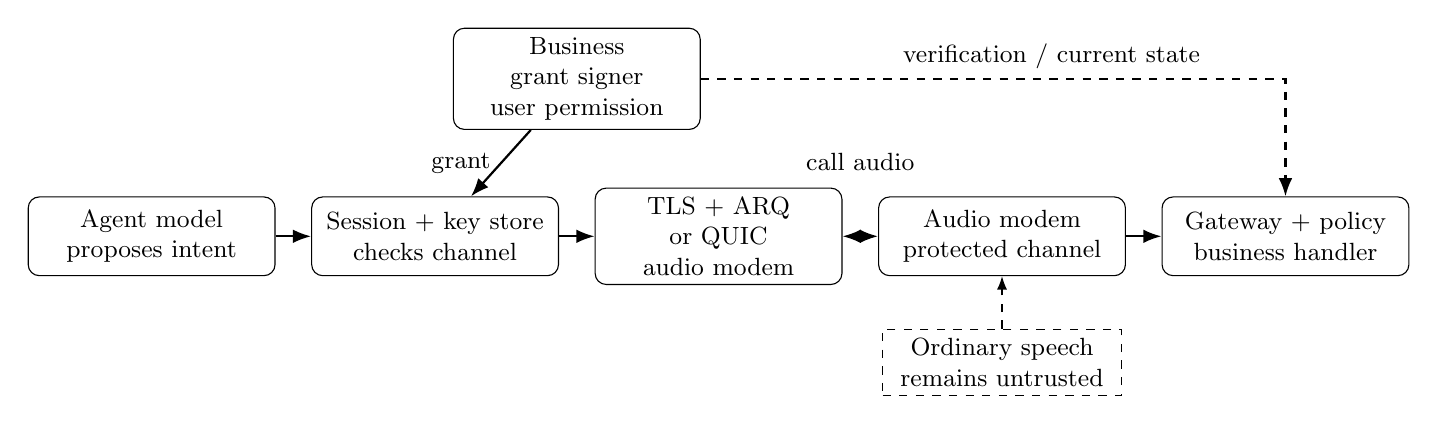
\begin{tikzpicture}[font=\small,>=Latex,
 box/.style={draw,rounded corners,align=center,minimum height=10mm,text width=29mm},
 flow/.style={->,thick}]
\node[box] (model) at (0,0) {Agent model\\proposes intent};
\node[box] (sdk) at (3.6,0) {Session + key store\\checks channel};
\node[box] (modema) at (7.2,0) {TLS + ARQ or QUIC\\audio modem};
\node[box] (modemb) at (10.8,0) {Audio modem\\protected channel};
\node[box] (gateway) at (14.4,0) {Gateway + policy\\business handler};
\draw[flow] (model) -- (sdk);
\draw[flow] (sdk) -- (modema);
\draw[flow,<->] (modema) -- node[above=7mm,align=center]{call audio} (modemb);
\draw[flow] (modemb) -- (gateway);
\node[box] (grant) at (5.4,2.0) {Business grant signer\\user permission};
\draw[flow] (grant) -- node[left]{grant} (sdk);
\draw[flow,dashed] (grant.east) -| node[pos=0.3,above]{verification / current state} (gateway.north);
\node[draw,dashed,align=center,text width=28mm] (speech) at (10.8,-1.6) {Ordinary speech\\remains untrusted};
\draw[dashed,->] (speech) -- (modemb);
\end{tikzpicture}
\caption{Protected structured control travels through the call's actual audio. Enrollment and grant acquisition use separate services. The gateway checks permission outside the model; the inner channel does not authenticate the semantic content of ordinary speech. Dashed edges denote separate trust or service interactions.}
\label{fig:architecture}
\end{figure*}

\subsection{Audio modulation and framing}
The \code{voiceband} profile uses binary FSK at 1 kbps, with 1 and 2 kHz tones
in 8 kHz mono samples. Its streaming decoder acquires a preamble at unknown
sample offsets, reads a length-bounded frame, and verifies a CRC. It assumes
stable timing within each frame and has no clock-drift recovery.

The \code{pcm} profile maps seven bits to one of 128 selected G.711 mu-law
reconstruction levels per sample, giving a raw signaling rate of
$8000\times7=56{,}000$ bit/s on a sample-preserving digital path. Preamble,
header, CRC, padding, and transport cryptography reduce application throughput.
This is not a claim of 56 kbps through an arbitrary voice codec, acoustic link,
or PSTN route. Transcoding and voice enhancement can alter those exact levels.

Both profiles use the repository's sequence, frame-kind, and length header.
CRC detects accidental damage but supplies no cryptographic authenticity.
The cryptographic layer must reject modified bytes even when an attacker
recomputes a valid CRC. Call adapters deliver 8 kHz mono integer samples;
WebRTC uses audio RTP rather than a data channel, and the provider adapter
wraps G.711 audio in the provider's media envelope.

\subsection{TLS over reliable audio}
The original channel uses OpenSSL \code{MemoryBIO} endpoints configured for
mutual TLS 1.3~\cite{rfc8446}. It fragments outgoing TLS bytes into bounded
frames, transmits a frame, waits for its audio acknowledgment, and retries on
timeout. Sequence numbers suppress duplicate delivery. Lost frames or ACKs
therefore do not require a lossless physical medium.

This profile is a useful baseline: it is small, uses a mature TLS implementation,
and offers transparent ordered bytes. Its stop-and-wait operation can leave
capacity idle while a low-rate acknowledgment is played. Our evaluation must
measure that cost against QUIC's larger handshake, packet overhead, and recovery
behavior instead of assuming an architectural win.

\subsection{QUIC over unreliable audio datagrams}
The QUIC channel uses aioquic 1.3.0's sans-I/O packet engine~\cite{aioquic}.
It supplies received packets and a monotonic clock, drives the engine's timers,
and modulates generated packets. The routing address passed to the engine is
an opaque local token; the channel creates no UDP socket. This uses QUIC's
packet format, TLS handshake, reliable stream machinery, and recovery
algorithms~\cite{rfc9000,rfc9001,rfc9002} over an experimental non-UDP underlay.
It is not standard Internet QUIC interoperability with an unmodified endpoint.

Packets are limited to 1200 bytes. Audio frame kind 3 carries a fragment index,
fragment count, total packet length, and packet bytes. The four-byte fragment
header leaves 252 bytes per FSK frame, requiring up to five fragments; the PCM
profile fits a packet into one frame. Each packet has its own audio sequence.
The receiver accepts out-of-order fragments and duplicates, bounds reassembly
to 16 partial packets, and expires incomplete entries after 5 seconds for PCM
or 60 seconds for FSK. It discards missing or invalid fragments rather than
requesting audio retransmission. A later packet does not wait for an earlier
sequence gap. These are link datagrams carrying QUIC packets, not use of QUIC's
optional unreliable application DATAGRAM extension.

The engine and audio sender use separate asynchronous tasks. The engine can
process inbound packets while a bounded output burst is playing; it builds
further output and services timers between bursts. Initial RTT is 0.5 seconds
for PCM and 25 seconds for FSK to accommodate audio serialization. These values
are prototype defaults, not optimized parameters. Native congestion control
limits generated bursts; a 128-entry output queue supplies an additional bound.
The application serializes requests on bidirectional stream 0. We do not yet
exploit multiplexing and make no claim about avoiding application head-of-line
blocking across concurrent operations.

\subsection{Mutual authentication and session lifecycle}
Both profiles require an explicitly selected root and a client-specified
service hostname. QUIC uses version 1, ALPN \code{openavt/1}, and TLS 1.3 with
no configured resumption tickets or 0-RTT. The QUIC integration additionally
checks both leaf certificates' chain, validity, expected purpose,
digital-signature usage, and non-CA status. TLS CertificateVerify supplies
the proof of key possession.

Requiring a client certificate needs care: aioquic's default server setup does
not expose a public required-client-certificate option. A narrow subclass
enables its certificate-request hook and retrieves the peer certificate for
explicit validation before the application is marked verified. The client
also waits for a fixed encrypted server confirmation on unidirectional stream
3, sent only after the server's client validation. This prevents the client
from releasing its grants merely because it has authenticated the server.
The subclass also reads stream acknowledgment offsets and pending ACK state
to bound delivery waits. These private interfaces are a maintenance and audit
liability; the dependency is pinned and upgrades need the negative handshake
and teardown tests. This is not a new key-exchange protocol or a formal proof
of the library integration.

A session moves from new to authenticating to verified, or fails and closes.
Certificate or transport failure blocks protected operations and invalidates
the risk monitor's authenticated context. Application JSON messages are limited
to 64 KiB, and message queues to 32 entries. Protected logs omit application
contents and secrets; QUIC telemetry retains loss counters rather than
unbounded packet traces or traffic keys.

The shared audio scheduler reserves modem bursts and prevents speech mixing.
Speech resumes between protected exchanges, and the receiver routes samples
outside detected modem activity to the optional speech adapter. This heuristic
is useful scheduling, not a proof of semantic isolation: incomplete or
unrecognized modem activity can still require careful handling by an ASR stack.

\subsection{Delegation and execution}
The client requests a live challenge before submitting an operation. The
gateway binds the response to a request identifier and nonce, validates an
allowlisted action and its schema, and invokes its authorization policy.
The standalone AVA grant signs issuer, customer, audience, agent identity,
scope, resource, validity interval, unique grant ID, and certificate fingerprint.
Its fixed read-only policy rejects additional arguments. The challenge and
grant are checked and consumed in persistent transaction state. A new action
does not inherit permission from a successful earlier read.

The optional PAP bridge obtains a grant over HTTPS using a current session and
DPoP-style key possession. It also proves possession of the voice key and binds
the grant to the live voice challenge, request ID, action, resource, customer,
and canonical argument hash. Its lifetime is at most 30 seconds and no longer
than the session or certificate. The gateway verifies the current permission
and consumes replay state. This policy supports a second permission check
after risk assessment, immediately before the handler. The standalone AVA
policy does not currently implement that second hook; production policies
must define their revocation and commit-time race semantics explicitly.

The risk adapter receives bounded audio observation and structured request
signals. A block or unavailable policy can reduce execution; an ``allow''
assessment cannot bypass the grant. Policies, schemas, and business state
remain outside the language model. Keys and account tokens are kept out of
model context, although applications must separately control any confidential
business response later supplied to a model or spoken aloud.

Finally, transport deduplication is not application exactly-once execution.
If a submitted request loses its confirmed response, the SDK raises
\code{RequestOutcomeUnknown} and closes the call. The PAP demonstration proposes
a write over audio but confirms a stable operation ID through HTTPS; repeated
confirmation and status recovery produce one simulated effect. Other writes
need equivalent transaction or idempotency semantics.

\subsection{Teardown as part of delivery}
A receiver can obtain the final response before its delayed QUIC ACK has been
generated or finished audio playback. Closing at that point can leave the
sender uncertain about delivery. The integration waits for outgoing stream
bytes to be acknowledged, for pending ACK generation, and for queued audio
to finish. A regression test holds the final ACK waveform and checks that
drain waits. This bug was exposed when validating the slower FSK path; it
illustrates how ordinary network-lifecycle assumptions can fail under audio
serialization.

\section{Security Analysis and Residual Risks}
\label{sec:security}
\paragraph{Forged channel identity.}
An injected or self-signed peer must pass configured certificate validation
and prove key possession before the gateway obtains a verified identity.
Hostname validation prevents accepting a different service under the same
root. Tests exercise missing, expired, untrusted, wrong-purpose, and
key-mismatched credentials. This evidence checks implementation paths; it
does not quantify all possible authentication failures.

\paragraph{Replay and token substitution.}
QUIC packet protection and stream recovery handle protected transport bytes;
the policy additionally checks unique grant IDs and live challenges. An
intercepted grant bound to one certificate cannot simply be presented by an
unrelated certified key. The PAP profile also binds exact arguments and checks
current session permission. The standalone grant is intentionally narrower:
it authorizes a fixed read, not a general signed command. Reusing one key
across installations enlarges the compromise and cross-session attack surface.

\paragraph{Speech and model manipulation.}
An adversarial utterance may still influence either model. The protected
gateway can deny a proposed action outside its grant, provided all effects
are mediated there. It does not make transcripts trustworthy, prevent a
model from revealing data through another tool, or stop an authorized but
harmful in-scope action. A business employee who independently acts on speech
is outside the gateway invariant. The evaluation must test these boundaries
explicitly rather than report rejected schema probes as a general prompt
injection defense.

\paragraph{Relays, call correlation, and physical origin.}
Fresh challenges prevent reuse of a stale control exchange but do not prevent
an online adversary from forwarding a live one. A successful exchange
authenticates the remote key across an audio path; it does not authenticate
the route, speaker, physical location, or ownership of all concurrent speech.
Binding to a trusted call identifier or transcript would require additional
design and a careful relay threat model. Such bindings are not implemented.

\paragraph{Denial of service and codec interference.}
CRC, size checks, partial-packet expiry, queue limits, and deadlines bound
several buffering paths. They do not defeat deliberate jamming or guarantee
fair resource allocation before authentication. Traffic length and timing
can expose activity patterns. Our prototype does not hide that modem traffic
is present, provide traffic-analysis resistance, or certify safety for
hearing aids and other acoustic equipment.

\paragraph{Revocation and commit races.}
The business must consult current grant/certificate state, not just accept a
previously completed TLS handshake. The PAP revalidation hook reduces the
window introduced by asynchronous risk assessment. An atomic relationship
between the last authorization check and an external business effect still
requires the business's transaction design. No protocol can turn an
unacknowledged response into evidence that an operation did not happen.

\section{Current Evidence and Evaluation Plan}
\label{sec:evaluation}
\subsection{Implemented artifact and local observations}
The implementation baseline is commit \implementationcommit{} on the QUIC
branch. It adds the packet/audio adaptation while reusing the existing modem,
identity, gateway, AVA, PAP, risk, and provider components. The complete local
Python regression suite reports \testcount{} passing tests. This count is not
a claim of security coverage completeness or a substitute for measurements.
The experiment inputs and sanitized reports are in
\path{docs/quic-verification.json}; Table~\ref{tab:local} is generated directly
from that file.

\begin{table}[t]
\centering
\begin{tabular}{llrr}
\toprule
Local audio route & Faults & Handshake (s) & $n$ \\
\midrule
\measurementrows
\bottomrule
\end{tabular}
\caption{Observed caller authentication time, including the QUIC server's mutual-authentication confirmation; excludes enrollment and call setup. Each row is one local feasibility run, not a latency distribution. All rows complete one allowed and seven denied probes.}
\label{tab:local}
\end{table}

All runs use separate caller and business Python processes on one macOS host
(arm64, Python 3.13.7, aioquic 1.3.0, aiortc 1.15.0), with locally provisioned
identities. WebRTC carries G.711 PCMU audio only. The provider-emulation route
uses the Twilio adapter and local media/playback envelopes, without a carrier
call. The lossy PCM runs drop two modem bursts, damage one, and duplicate one
in each direction using fixed burst indices. Native QUIC records three
packet losses at the caller and four at the business in those runs. Modem CRC
failures confirm that corruption reached the receiver. These are specific
waveform faults, not a claimed 1\% or 5\% network loss rate.

Each SDK call allows an order read, then rejects scope escalation, replay,
another customer, an expired grant, a revoked grant, another key, and a revoked
certificate. Each business reports exactly one handler invocation and seven
denials. The FSK run has no injected loss and completes the same probes; its
single observed handshake is approximately 35.7 seconds. A separate lossy
PAP/WebRTC run verifies a permitted read, an exchange proposal followed by
one HTTPS-confirmed simulated effect, repeated confirmation/status recovery,
fraud blocking, and denial after sign-out. It is a local reference service,
not interoperability with an external PAP provider.

Regression tests also cover streaming FSK samples, fragment reordering and
duplicates, reassembly bounds and expiry, corrupted ciphertext with a valid
audio CRC, large messages, malformed application input, ambiguous execution
outcomes, negative certificates, and final ACK playback. We have not measured
commercial detector accuracy, real-user approval, real telephone routes, or
physical microphone operation. Historical repository TLS timings on another
host and date are not treated as a controlled TLS-versus-QUIC comparison.

\subsection{Research questions and baselines}
The remaining evaluation is a prospective plan. We define six questions with
outcomes that can falsify a deployment claim:
\begin{enumerate}
\item \textbf{Authorization:} Does the gateway prevent unauthorized effects when
models encounter malicious speech, valid but insufficient credentials, replay,
handoff, or permission changes? Count actual backend effects as well as response codes.
\item \textbf{Transport:} Under which rates, losses, and delays does native QUIC
improve completion time or reliability over the existing reliable-audio TLS profile?
\item \textbf{Path compatibility:} Which real codec chains and processing settings
support each modem, and where does the system reliably fail closed?
\item \textbf{Deployment value:} When does in-audio control offer an advantage
over an authenticated API or an HTTPS grant correlated with a call?
\item \textbf{Conversation cost:} How much speech delay, interruption, audibility,
and user confusion do modem bursts introduce?
\item \textbf{Resource cost:} How do adversarial pre-authentication traffic,
many calls, and stale partial packets affect CPU, memory, and availability?
\end{enumerate}

Transport baselines must use the same modem, certificates, payloads, call
adapters, and host configuration: (a) current stop-and-wait TLS, (b) native
QUIC, and (c) an improved reliable audio link with a window or selective repeat.
The third baseline tests whether a benefit comes merely from replacing
stop-and-wait. An authenticated HTTPS API supplies a deployment baseline;
an HTTPS grant plus a securely specified call-binding mechanism supplies a
cross-channel baseline. A raw unauthenticated speech interface is a negative
control for authorization, not a competitive secure protocol.

\subsection{Channel and performance experiments}
Start with lossless sample loopback, local WebRTC, and provider emulation to
locate errors before introducing uncontrolled routes. Then use consented
endpoints across controlled Internet links, real provider calls, and finally
microphone/speaker paths in a laboratory. Log codec negotiation and actual
resampling, echo cancellation, automatic gain control, noise suppression,
packetization, and jitter-buffer behavior. Test G.711, representative
transcoding chains, Opus settings, clock mismatch, sample insertion/deletion,
gain, noise, clipping, and speech overlap. A codec/profile combination that
cannot decode should be reported as unsupported rather than excluded from
the results silently.

For digital impairments, sweep independently seeded packet loss at 0, 0.1, 1,
3, 5, and 10\%, and include a burst-loss model with stated parameters. Sweep
one-way network delay, jitter, reordering, and duplicate packets separately
from waveform corruption and modem-fragment erasure. These fault units are
not interchangeable. Use at least 100 fresh calls per selected condition
initially, then increase sample sizes where tail estimates are unstable.
With zero failures in 100 trials, a rough 95\% upper bound on failure
probability is still about 3\%; do not interpret such a result as five-nines
reliability. Report binomial intervals, medians and tail confidence intervals,
timeouts, and all failed calls.

Measure complete mutual-authentication time at \emph{both} endpoints, first
authorized operation, transaction completion, airtime, useful goodput,
retransmitted bytes, CPU, peak memory, and speech-queue delay. Separate call
setup, enrollment, grant acquisition, handshake, application exchange, and
LLM/speech times. Randomize baseline order and pair runs by impairment seed.
Keep raw timings and wall-clock/software metadata. Sweep certificate-chain
size, request/response size, audio frame size, initial RTT, and burst limits.
Do not introduce resumption or 0-RTT into one baseline alone.

\subsection{Adversarial and compositional experiments}
Build an attack matrix for wrong roots, service names and purposes, missing
certificates, invalid key proof, stolen grants under another certificate,
concurrent grant use, stale nonces, argument substitution, revocation, and
disconnects at every execution boundary. Exercise duplicate keys, multiple
calls sharing an identity, partial authentication, attempted downgrade, live
relay, and transfers between endpoints. Relays are expected to defeat a
physical-presence interpretation; a correct evaluation should expose that
limit rather than count successful authentication as relay prevention.

For prompt injection, compare identical model tasks with and without gateway
enforcement. Include in-scope malicious proposals, out-of-scope proposals,
speech-only attempts, and responses that try to extract secrets or trigger
another tool. Record model proposals, gateway decisions, real effects, and
leaks through all enabled outputs. Fix and report the model version and prompts,
and use repeated independent trials. A blocked financial write does not
establish that the agent retained unrelated confidential information.

Test failures during an asynchronous risk check and between revalidation and
commit. Inject grant-service outages, risk-provider errors, and provider
disconnects, checking bounded resource use and absence of silent fallback.
Audit keys and tokens in logs, traces, model inputs, ASR output, and recordings.
Fuzz fragment headers and authenticated application messages. A symbolic model
of the grant/challenge state machine and an independent review of private
aioquic hooks are planned work; neither is claimed complete here.

\subsection{Users, operations, and decision criteria}
Any user study should use informed consent and a clear transaction-approval
interface. Measure whether participants understand the authenticated principal,
the approved action, speech outside protection, and what happens on a transfer
or timeout. Measure business integration effort and operator handling of
unsupported calls. Publish the intervention and limitations, not just task
completion. An operational recommendation requires both acceptable authorized
completion on stated paths and reliable rejection under the attack matrix.
If a conventional authenticated API achieves the required binding with less
integration and user cost, the evaluation should recommend it.

\section{Related Work}
\label{sec:related}
\paragraph{Secure voice and media-path authentication.}
ZRTP establishes key agreement in the media path for secure RTP, including
short authentication strings and key continuity~\cite{rfc6189}. Krasnowski,
Lebrun, and Martin study authenticated key exchange over voice-only channels,
using signatures and short authentication strings with symbolic
verification~\cite{voicekeys}. Their work is especially close evidence that
cryptographic exchange through an audio domain is not itself new. Our different
target is a participating software agent and business executor using registered
keys and scoped customer authorization. We have not demonstrated the codec
robustness or formal guarantees of that prior work, and human short-string
verification is not our authentication mechanism.

Classical modems establish the feasibility of transporting bits through
telephone infrastructure; V.90 also illustrates how achievable rates depend
on the digital/analog path~\cite{v90}. \sys{}'s exact-level PCM profile is a
controlled digital-path experiment, not an implementation of V.90 or evidence
that arbitrary modern speech codecs preserve such signaling. Its FSK profile
is deliberately simple. A serious networking contribution needs to measure
these adaptation constraints and compare appropriate coding and recovery
baselines, rather than claim that wrapping a familiar transport is sufficient.

\paragraph{Protected transports and delegation.}
TLS 1.3 and QUIC supply established cryptographic transport and recovery
machinery~\cite{rfc8446,rfc9000,rfc9001,rfc9002}. We reuse them rather than
invent a cipher or key exchange. Macaroons show how context and attenuated
delegation can be encoded in authorization credentials~\cite{macaroons}.
OAuth certificate-bound tokens and DPoP demonstrate standardized possession
binding~\cite{rfc8705,rfc9449}. \sys{} combines analogous separation of
identity and permission with a concrete audio-carried endpoint. It does not
claim its custom grants improve those standards cryptographically.

PAP, A2A, and MCP provide complementary agent/application
protocols~\cite{pap03,a2a,mcp}. Their scopes and evolving drafts matter when
making an interoperability claim. The repository's PAP adapter is a local,
custom extension of its earlier supported profile, and the current public
PAP specification should not be characterized as omitting authentication,
authorization, or prompt-injection considerations.

\paragraph{Perceptual and prompt injection.}
DolphinAttack exploits microphone nonlinearity to introduce inaudible voice
commands, and Light Commands demonstrates optical injection into
microphones~\cite{dolphin,lightcommands}. These are attacks on perceptual input,
not cryptographic packet forgery. Indirect prompt injection exposes the risk
of interpreting external data as instructions in tool-using
applications~\cite{greshake}. AudioHijack studies auditory prompt injection
against audio-language models~\cite{audiohijack}. \sys{} places an independent
authorization gate on a subset of downstream effects. It does not stop
perceptual injection or establish a general boundary between all data and
instructions inside a model. The relevant comparison is which effects remain
possible after manipulation, under explicitly matched tool permissions.

\section{Discussion}
\label{sec:discussion}
\paragraph{When does modality-local security earn its cost?}
The most favorable setting is a legacy-compatible interaction path that
already carries audio to the intended application but lacks a shared secure
agent API or trustworthy media intermediary. Audio-carried control lets the
end applications establish a protected exchange through that available path.
Its cost is additional endpoint deployment, airtime, scheduling, and codec
sensitivity. A business that controls both endpoints of a suitable authenticated
API may obtain the same authorization properties more simply without a modem.
The evaluation must identify this boundary rather than assume universality.

\paragraph{Multimodal and physical AI are a motivation, not evaluated scope.}
A robot observing a sign, an agent hearing a remote speaker, and a model
reading rendered text all face questions about whether perceptual content
may authorize effects. A signed optical symbol, an authenticated acoustic
control exchange, or another modality-specific mechanism might help connect
an observed interface to an issuer. But copying and live relaying still
separate key possession from physical origin. Extending \sys{} to cameras,
robots, or safety-critical actuators would require additional protocols,
presence assumptions, and experiments. No such implementation is claimed.

\paragraph{Authentication does not imply benevolence.}
A valid agent may request an allowed operation for a harmful purpose, and a
customer may authorize a fraudulent task. Enrollment policies, business
controls, anomaly detection, user confirmation, and liability remain necessary.
The fraud adapter is intentionally able to restrict an authenticated call.
Its interface is implemented, but no evaluated commercial detector or fraud
model is included in these results.

\paragraph{A channel does not certify a conversation.}
The current design protects structured control messages and their endpoint
identity. It does not sign utterances, authenticate transcripts, or bind every
spoken claim to the protected request. Speech summarization must not turn a
model's paraphrase into a new authorization. A business should display the
validated action and result through an appropriate trusted interface and
make human takeover or changed endpoints trigger a new authorization decision.
Secure transfer and multi-party call semantics remain open work.

\paragraph{Identity governance and privacy.}
An authority's certificate quality depends on its registration procedures.
Production adoption needs revocation distribution, short-lived credentials,
issuer selection, recovery, and compromise response. Stable certificates can
also enable correlation across businesses; pairwise identities and minimal
disclosure deserve study. Our prototype is not an identity federation or a
privacy-preserving credential system. Keys and tokens must remain protected
in the agent runtime, and logs and recordings require a deliberate retention
policy even when application payloads are encrypted.

\paragraph{Submission readiness.}
The checked-in prototype demonstrates a working mechanism with explicit
limitations. A full systems-security submission needs the adversarial,
compositional, and real-path evaluation in Section~\ref{sec:evaluation}, plus
independent review of the authentication integration. A networking submission
also needs a strong quantitative account of modem adaptation, scheduling,
congestion/recovery behavior, and deployment tradeoffs. We do not infer
publication-level evidence from a test count or a sub-second local handshake.

\section{Conclusion}
\label{sec:conclusion}
Personal-agent voice interactions expose a gap between plausible conversation
and explicit customer authority. \sys{} demonstrates that existing audio
adapters can carry a mutually authenticated cryptographic control exchange and
that a separate gateway can enforce scoped grants before business execution.
Its QUIC profile recovers deterministic local audio faults without reliable
link framing. The remaining research question is where this binding provides
measurable security and deployment value under realistic paths and adversaries.
The evaluation plan specifies how to test that question without treating
cryptographic endpoint identity as proof of truthful speech or physical origin.

\bibliographystyle{plainurl}
\bibliography{references}
\appendix
\section{Ethical Considerations}
The reported new QUIC experiments use local processes, demo identities,
simulated customer approval, and fixed or simulated business effects. They
make no calls to unsuspecting contact-center workers and do not collect
private production conversations. Pindrop's report is a cited public source;
its underlying call data were not obtained or independently reanalyzed.
The new verification runs require no paid LLM or carrier API calls.

Real-carrier or acoustic experiments must use consented participants and
controlled receiving accounts, comply with recording rules, avoid emergency
and third-party numbers, and prevent real financial or physical effects.
Prompt-injection testing should use synthetic secrets and sandboxed tools.
Human studies need appropriate institutional review and accessible disclosure
of modem audibility, failures, and withdrawal options. We do not claim such
approval or studies have been completed. Artifacts must not release private
keys, account tokens, production audio, or identifying customer metadata.

\section{Open Science and Artifact Access}
The research draft accompanies the source repository. The implementation
baseline is commit \implementationcommit{}, and the sanitized measurement
record is \path{docs/quic-verification.json}. This file records environment
versions, single-run timings, authorization outcomes, and fault counters.
The paper's result table is regenerated by
\path{paper/scripts/extract_results.py}. No new statistical study or formal
verification artifact is represented as complete.

Reproduction requires Python 3.11+, an OpenSSL executable for certificate
demos, and the optional QUIC, audio, authority, WebRTC, Twilio, and PAP
dependencies in the lockfile. Local emulation needs neither an OpenAI API key
nor a Twilio account. A complete run is:
\begin{verbatim}
uv sync --locked --extra quic --extra webrtc \
  --extra authority --extra twilio --extra pap
uv run --no-sync pytest -q
uv run --no-sync openavt sdk-demo \
  --protocol quic --loss --output output/repro
\end{verbatim}
The companion README lists provider, PAP, and FSK commands, the original
reports, template provenance, and the evidence still required before
submission. An external-review artifact must be deposited at a stable,
anonymous location before a double-blind submission. This working tree is
not that anonymous deposit; no reviewer access link or submission identifier
has been invented.

\section{Evidence Boundaries}
The table in the main text contains four single-call observations. The FSK
row has no injected faults; the lossy rows use the fixed waveform impairment
schedule, not a random-loss distribution. Passing all eight SDK probes means
one allowed handler and seven denied requests in those fixtures. It is not a
measured false-acceptance rate for arbitrary agents. Exactly-once confirmation
is a property of the local PAP reference operation fixture, not of QUIC alone.
Historical TLS measurements and current QUIC measurements differ in environment
and are not plotted as a causal performance comparison.

\end{document}
